%%% File: /inputs/parts/CONSCIOUS_ATTENTION.tex

%%% %%%%%%%%%%%%%%%%%%%%%%%%%%%%%%%%%%%%%%%%%%%%%%%%%%%%%%%%%%%%%%%%%%%%%%%%%%%%

Stanislas Dehaene and his colleagues have developed a computational model of consciousness that provides a practical framework for thinking about consciousness that is sufficiently detailed for much of what an engineer might care about in designing digital assistants~\cite{Dehaene2014}. Dehaene's work extends the {\it{Global Workspace}} Theory of Bernard Baars~\cite{Baars1988}. Dehaene's version of the theory combined with Yoshua Bengio's concept of a {\it{consciousness prior}} and deep reinforcement learning~\cite{MnihetalCoRR-13,NairetalCoRR-15} suggest a model for constructing and maintaining the cognitive states that arise and persist during complex problem solving~\cite{BengioCoRR-17}.

Global Workspace Theory accounts for both conscious and unconscious thought with the primary distinction for our purpose being that the former has been selected for attention and the latter has not been so selected. Sensory data arrives at the periphery of the organism. The data is initially processed in the primary sensory areas located in posterior cortex, propagates forward and is further processed in increasingly-abstract multimodal association areas. Even as information flows forward toward the front of the brain, the results of abstract computations performed in the association areas are fed back toward the primary sensory cortex. This basic pattern of activity is common in all mammals.

Humans have a large frontal cortex that includes machinery responsible for conscious awareness and that depends on an extensive network of specialized neurons called {\it{spindle cells}} that span a large portion of the posterior cortex allowing circuits in the frontal cortex to sense relevant activity throughout this area and then manage this activity by creating and maintaining the persistent state vectors that are necessary when generating extended narratives or working on complex problems that require juggling many component concepts at once. Figure~{\urlh{#fig_Global_Workspace_Conscious_Attention}{\ref{fig_conscious}}} suggests a neural architecture combining the idea of a global workspace with that of an attentional system for identifying relevant input.

%%% %%%%%%%%%%%%%%%%%%%%%%%%%%%%%%%%%%%%%%%%%%%%%%%%%%%%%%%%%%%%%%%%%%%%%%%%%%%%

%%% Figure~{\urlh{#fig_Global_Workspace_Conscious_Attention}{\ref{fig_conscious}}}
\begin{figure}
%
  \begin{center} 
%    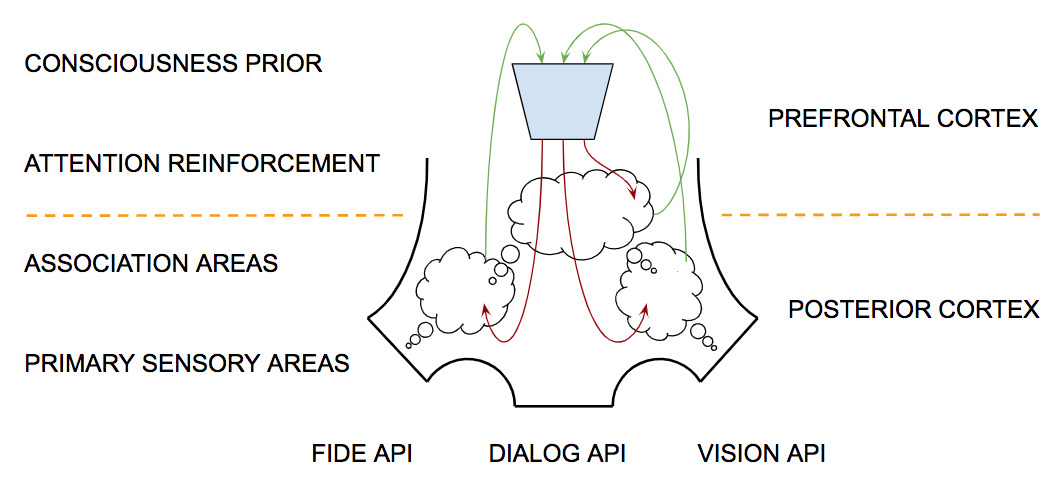
\includegraphics[width=530pt]{./figures/Global_Workspace_Conscious_Attention.png} % 1063 × 487 pixels
    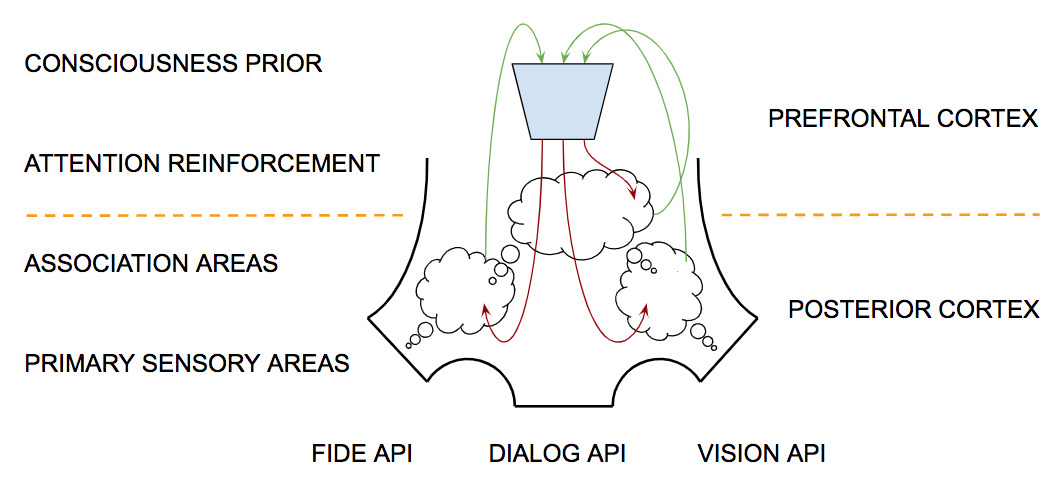
\includegraphics[height=130pt]{./figures/Global_Workspace_Conscious_Attention.png} % 1063 × 487 pixels
  \end{center}
%
  \caption{The basic capabilities required to support conscious awareness can be realized in a relatively simple computational architecture that represents the apprentice's global workspace and incorporates a model of attention that surveys activity throughout somatosensory and motor cortex, identifies the activity relevant to the current focus of attention and then maintains this state of activity so that it can readily be utilized in problem solving.  In the case of the apprentice, new information is ingested into the model at the system interface, including dialog in the form of text, visual information in the form of editor screen images, and a collection of programming-related signals originating from a suite of software development tools. 
%
Single-modality sensory information feeds into multimodal association areas to create rich abstract representations. Attentional networks in the prefrontal cortex take as input activations occurring throughout the posterior cortex. These networks are trained by reinforcement learning to identify areas of activity worth attending to and the learned policy selects a set of these areas to attend to and sustain. This attentional process is guided by a prior that prefers low-dimensional thought vectors corresponding to statements about the world that are either true, highly probable or very useful for making decisions. Humans can sustain only a few such activations at a time. The apprentice need not be so constrained.}
%
  \label{fig_conscious}
%
\end{figure}

%%% %%%%%%%%%%%%%%%%%%%%%%%%%%%%%%%%%%%%%%%%%%%%%%%%%%%%%%%%%%%%%%%%%%%%%%%%%%%%

%%% Note: Consider adding a paragraph summarizing the engineer's view of consciousness that Dehaene [18], Dennett [19] and Graziano [33] espouse: conscious awareness is a form of attention; the sense of self is a consequence of feedback due to recurrent connections in the cortex [40]; and the fact that we report being conscious and engage in an internal dialogue is a consequence of the reciprocal connections between the generative and interpretative speech centers in the brain [23]. The title of Michael Graziano's article [34] in The Atlantic summarizes the view succinctly: "Consciousness is not mysterious: It's just the brain describing itself to itself".

%%% Note: Consider adding a paragraph summarizing the engineer's view of consciousness that Dehaene~\cite{Dehaene2014}, Dennett~\cite{Dennett91} and Graziano~\cite{Graziano2013} espouse: conscious awareness is a form of attention; the sense of self is a consequence of feedback due to recurrent connections in the cortex~\cite{Hofstadter2007}; and the fact that we report being conscious and engage in an internal dialogue is a consequence of the reciprocal connections between the generative and interpretative speech centers in the brain~\cite{Fernyhough2016voices}. The title of Michael Graziano's article~\cite{GrazianoATLANTIC-16a} in {\it{The Atlantic}} summarizes the view succinctly: "Consciousness is not mysterious: It's just the brain describing itself\emdash{}to itself".

%%% %%%%%%%%%%%%%%%%%%%%%%%%%%%%%%%%%%%%%%%%%%%%%%%%%%%%%%%%%%%%%%%%%%%%%%%%%%%%

%%% In Dehaene's theory, information about the external world enters the cortex through the thalamus and, with input from subcortical structures responsible for arousal and sleep, generates a signal marking the information available for examination. The raw sensory input is propagated to higher-level processing systems eventually reaching the prefrontal cortex where it is evaluated and selectively made available in short-term memory. The computations required for evaluation and selection can be modeled by attentional networks initialized with a prior that selects for suitably abstract features that maximize executive performance.

%%% The global workspace enables us to construct and maintain a complex composite representation in a serial fashion guided by attention. This can be accomplished using a form of persistent memory enabled by fast weights {\emdash{}} originally referred to as dynamic links in the work of Christoph von der Malsburg {\emdash{}} to manage a working memory in which information can be added, modified and removed, that supports associative retrieval and is implemented as a fully differentiable model and so can be trained end-to-end by gradient descent. Fast weights are used to store temporary memories of the recent past and provide a neurally plausible method of implementing the type of attention to the past that has recently proved helpful in sequence-to-sequence models. 

%%% %%%%%%%%%%%%%%%%%%%%%%%%%%%%%%%%%%%%%%%%%%%%%%%%%%%%%%%%%%%%%%%%%%%%%%%%%%%%

%%% Over the last few decades. Stanislas Dehaene at the Collège de France in Paris and Michael Graziano at Princeton University and their respective students and collaborators have developed computational models of consciousness that have made considerable progress in demystifying the confused thinking that characterizes much of the past philosophical discourse on consciousness. At the very least, I think it is fair to say that they provide a framework for thinking about consciousness that is satisfactory for almost anything an engineer might care about in designing digital assistants.

%%% Michael will be joining us next Tuesday to talk about his concept of an attention schema that facilitates human social interaction and addresses some of the issues that we will see later in building so-called theory-of-mind models that account for what other agents know. Several entries in the class discussion list summarize what you need to know about Dehaene's theory, including excerpts from his 2014 book, a succinct twenty-minute summary and a longer more-detailed lecture given by Dehaene. The twenty-minute summary here might be enough.

%%% Central to Dehaene's model of consciousness is the idea of maintaining a global workspace inspired by the work of Bernard Baars. The basic idea is that information is acquired and processed through our primary and secondary sensory systems, combined in increasingly abstract features in association areas to activate portions of episodic memory, and these activations feed into evaluative systems in the frontal cortex where attentional networks select memories in order to to construct complex representations in short-term memory.

%%% %%%%%%%%%%%%%%%%%%%%%%%%%%%%%%%%%%%%%%%%%%%%%%%%%%%%%%%%%%%%%%%%%%%%%%%%%%%%

%%% The cortical sheet, in addition to its layered structure, appears to be tiled with columnar structures referred to as cortical columns. Some neuroscientists believe that all of these columns compute the same basic function. However, there is considerable variation in cell type, thickness of the cortical layers, and the size of the dendritic arbors to question this hypothesis. The prefrontal cortex is populated with a type of neuron, called a spindle neuron, similar in some respects to the pyramidal cells found throughout the cortex, that allow rapid communication across the large brains of great apes, elephants, and cetaceans. Although rare in comparison to other neurons, spindle neurons are abundant and quite large in humans and apparently play an important role in consciousness and attentional networks.

These attentional networks are connected to regions throughout the cortex and are trained via reinforcement learning to recognize events worth attending to according to the learned value function. Using extensive networks of connections {\emdash{}} both incoming and outgoing, attentional networks are able to create a composite representation of the current situation that can serve a wide range of executive cognitive functions, including decision making and imagining possible futures. The basic idea of a neural network trained to attend to relevant parts of the input is key to a number of the systems that we'll be looking at.

%%% %%%%%%%%%%%%%%%%%%%%%%%%%%%%%%%%%%%%%%%%%%%%%%%%%%%%%%%%%%%%%%%%%%%%%%%%%%%%

%%% Fundamental to our understanding of human cognition is the essential tradeoff between fast, highly-parallel, context-sensitive, distributed connectionist-style computations and slow, serial, systematic, combinatorial symbolic computations. In developing the programmer's apprentice, symbolic computations of the sort common in conventional computing are realized using extensions that provide a differentiable interface to conventional memory and information processing hardware and software. Such interfaces include the Neural Turing Machine~\cite{GravesetalCoRR-14} (NTM), Memory Network Model~\cite{WestonetalCoRR-14,SukhbaataretalCoRR-15} and Differentiable Neural Computer~\cite{GravesetalNATURE-16} (DNC).

%%% %%%%%%%%%%%%%%%%%%%%%%%%%%%%%%%%%%%%%%%%%%%%%%%%%%%%%%%%%%%%%%%%%%%%%%%%%%%%

%%% Figure~{\urlh{#fig_Global_Workspace_Episodic_Memory}{\ref{fig_episodic}}}
\begin{figure}
%
  \begin{center} 
%    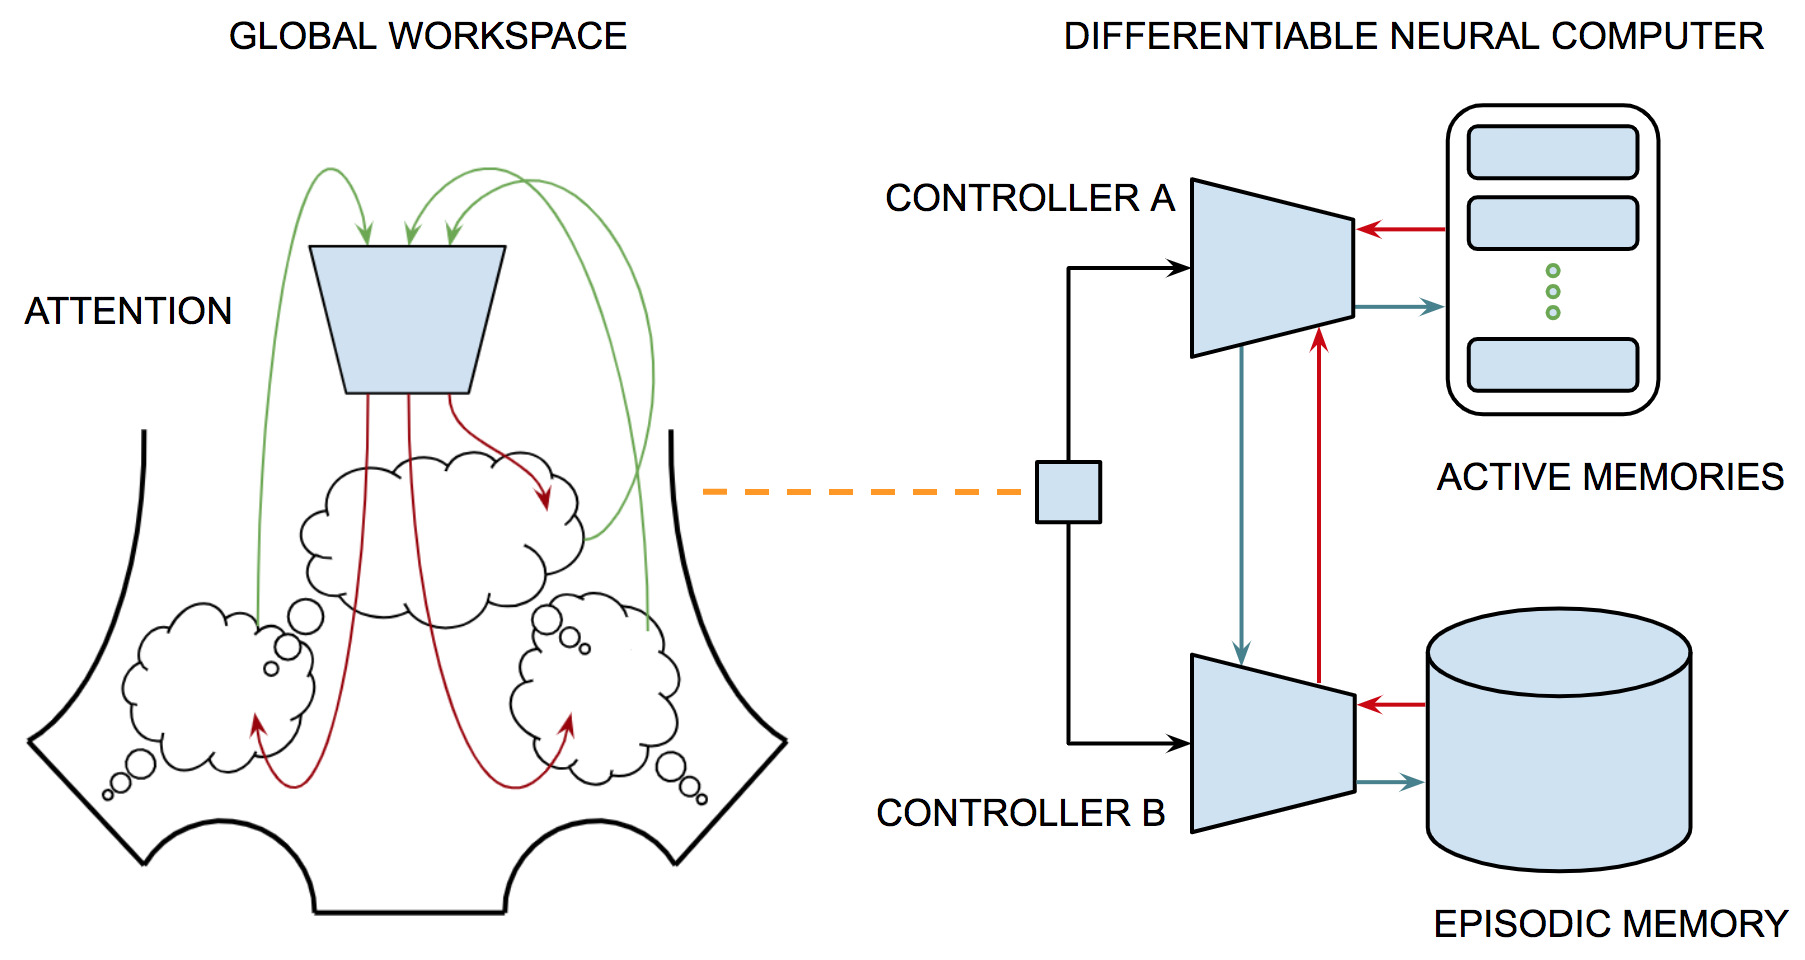
\includegraphics[width=590pt]{./figures/Global_Workspace_Episodic_Memory.png} % 1182 × 636 pixels
    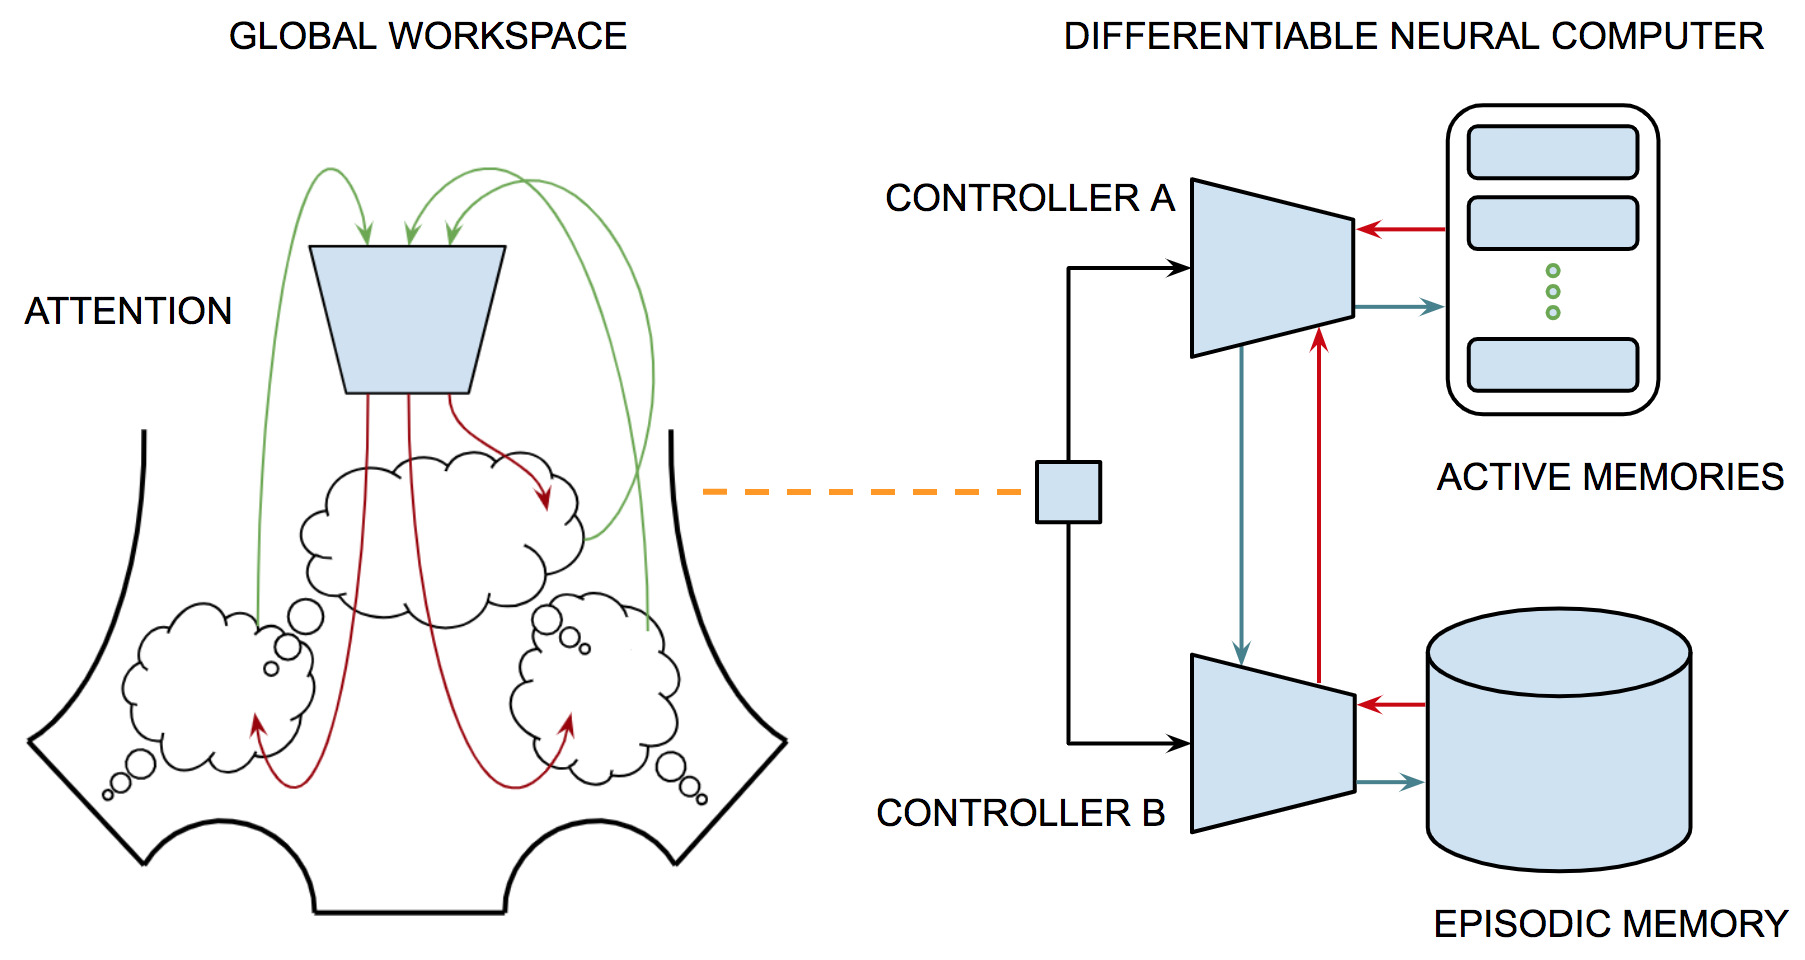
\includegraphics[height=150pt]{./figures/Global_Workspace_Episodic_Memory.png} % 1182 × 636 pixels
  \end{center}
%
  \caption{You can think of the episodic memory encoded in the hippocampus and entorhinal cortex as RAM and the actively maintained memories in the prefrontal cortex as the contents of registers in a conventional von Neumann architecture. Since the activated memories have different temporal characteristics and functional relationships with the contents of the global workspace, we implement them as two separate NTM memory systems each with its own special-purpose controller. Actively maintained information highlighted in the global workspace is used to generate keys for retrieving relevant memories that augment the highlighted activations. While the associative keys required to access locations only partially match locations, they can can still be used to guide attention allowing the NTM to recognize and even partially merge related locations. In general, locations in memory correspond to thought vectors that can be composed with other thought vectors to shape the global context for interpretation.}
%
  \label{fig_episodic}
%
\end{figure}

%%% %%%%%%%%%%%%%%%%%%%%%%%%%%%%%%%%%%%%%%%%%%%%%%%%%%%%%%%%%%%%%%%%%%%%%%%%%%%%

In their paper~\cite{GravesetalNATURE-16} in {\it{Nature}}, The authors note that "there are interesting parallels between the memory mechanisms of a DNC and the functional capabilities of the mammalian hippocampus. DNC memory modification is fast and can be one-shot, resembling the associative long-term potentiation of hippocampal CA3 and CA1 synapses. The hippocampal dentate gyrus, a region known to support neurogenesis, has been proposed to increase representational sparsity, thereby enhancing memory capacity: usage-based memory allocation and sparse weightings may provide similar facilities." See the discussion of neurogenesis as an algorithmic technique in {\urlh{box_patterns}{Box~\colorred{A}}}.

The global workspace summarizes recent experience in terms of sensory input, its integration, abstraction and inferred relevance to the context in which the underlying information was acquired. To exploit the knowledge encapsulated in such experience, the apprentice must identify and make available relevant experience. The apprentice's experience is encoded as tuples in an NTM that supports associative recall. We'll ignore the details of the encoding process to focus on how episodic memory is organized, searched and applied to solving problems.

%%% In the biological analog of an NTM the hippocampus and entorhinal region of the frontal cortex play the role of episodic memory and several subcortical circuits including the basal ganglia comprise the controller~\cite{OReillyetalLEABRA-16,OReillySCIENCE-06}. The controller employs associative keys in the form of low-dimensional vectors generated from activations highlighted in the global workspace to access related memories that are then actively maintained in the prefrontal cortex and serve to bias processing throughout the brain but particularly in those circuits highlighted in the global workspace. Figure~{\urlh{#fig_Global_Workspace_Episodic_Memory}{\ref{fig_episodic}}} provides a sketch of how this is accomplished in the apprentice architecture. 

%%% %%%%%%%%%%%%%%%%%%%%%%%%%%%%%%%%%%%%%%%%%%%%%%%%%%%%%%%%%%%%%%%%%%%%%%%%%%%%
